\chapter{\textit{Stage} proposto}
\label{chap:stage-proposto}

\section{Gestione aziendale degli \textit{stage}}\label{sec:stage-management}\noindent
% \texttt{Descrizione di come sono visti e gestiti in generale gli stage all'interno dell'azienda.}
M31 mostra molto interesse verso la creazione di rapporti con le nuove generazioni, questo avviene in diversi modi: tramite la M31 \textit{Academy} e tramite la partecipazione ai progetti di ``Ingegneria del \textit{Software}'' della laurea di informatica, come azienda proponente.\\
M31 \textit{Academy} è una sorta di settore aziendale dedicato alla realizzazione di progetti con studenti e studentesse universitarie o neo-laureati e neo-laureate. Ora come ora, l'azienda sta svolgendo progetti solo con studenti e studentesse universitarie, che prendono il ruolo di stagisti e stagiste, perciò passo a descrivere meglio come essi vengono gestiti.\\
L'influsso di stagisti e stagiste è principalmente dovuto alla partecipazione dell'azienda allo STAGE-IT, un evento promosso da Confindustria Veneto Est e l'Università di Padova, dove studenti e studentesse vengono introdotti a tre progetti che possono svolgere in azienda. M31 però offre una lista più numerosa di progetti, che vengono esposti quando gli studenti e studentesse contattano direttamente l'azienda.
Questi progetti, essendo numerosi, possono essere di vario tipo.
Alcuni pongono gli stagisti e stagiste in un progetto su cui l'azienda sta già lavorando.
Mentre altri, come quello che ho scelto io, servono all'azienda per esplorare nuove tecnologie o per prepararsi per un progetto aziendale che non ha ancora avuto modo di iniziare.

\section{Descrizione progetto}\label{sec:project-description}\noindent
% \texttt{Esposizione del problema affrontato dal mio progetto di stage.}
Il progetto di \textit{stage} consiste nella realizzazione di un'applicazione per l'analisi di dati tramite tecniche di \gls{machinelearning} e di \gls{deeplearning}; in particolare, per l'analisi di segnali elettrocardiografici, tramite elettrocardiogrammi.\\
Questo progetto di \textit{stage} serve all'azienda per prepararsi ad un progetto che si aspettano di affrontare in futuro, collaborando insieme ad un'azienda con cui sono attualmente in comunicazione.\\
Questo progetto vede come \textit{focus} principale la gestione di grandi quantità di dati, sotto forma di migliaia di \textit{file} contenenti segnali elettrocardiografici e altre informazioni sui pazienti.
Questi dati, facenti parte di un \gls{dataset}, vengono utilizzati all'interno di un programma per addestrare \glslink{neuralnetwork}{reti neurali artificiali}, ovvero di modelli che cercano di replicare il funzionamento del cervello umano.
Questi dati non possono subire modifiche inaspettate quando vengono inseriti nel processo di addestramento.
Inoltre, questi dati devono essere gestiti in modo efficiente, in modo da non caricare tutto all'interno della \gls{ram}, come viene generalmente fatto nel caso di \textit{dataset} di piccole dimensioni, così da non subire limitazioni di \textit{hardware}.\\
In secondo luogo, il progetto vede anche l'effettivo addestramento e valutazione di vari tipi di reti neurali artificiali, sia con lo scopo di testare, che di esplorare quali sono le tecniche migliori per l'analisi di elettrocardiogrammi.
\begin{figure}[H]
    \centering
    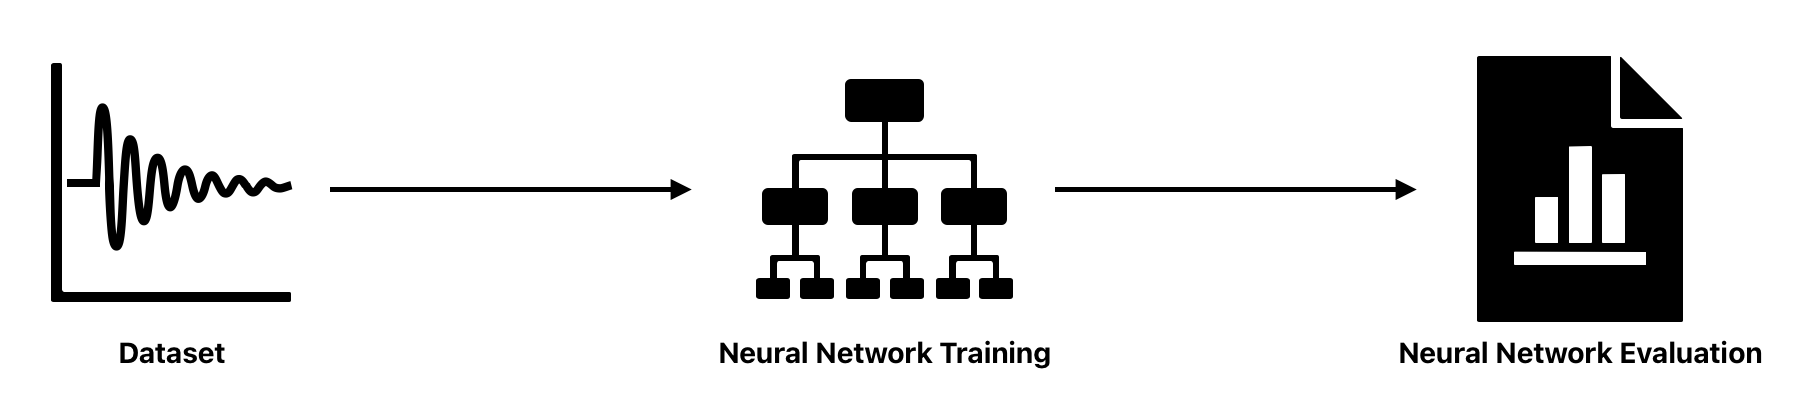
\includegraphics[alt={Rappresentazione dei punti principali del progetto}, width=0.9\columnwidth]{img/desc_proj.png}
    \caption{\centering Rappresentazione dei punti principali del progetto}
    \label{fig:desc-proj}
\end{figure}

\newpage

\section{Obiettivi}\label{sec:objectives}\noindent
%\texttt{Lista degli obiettivi da completare che riguardano il prodotto del mio operato durante lo stage, quindi quello che l'azienda vuole ottenere.}\\
Il progetto di \textit{stage} era definito da alcuni obiettivi richiesti dall'azienda, ognuno di essi era contrassegnato con una certa importanza; questa può rientrare in una dei tre seguenti tipi:
\begin{itemize}
    \item \textbf{Obbligatorio:} indica un obiettivo primario richiesto dal committente, il suo completamento non è negoziabile
    \item \textbf{Desiderabile:} indica un obiettivo non vincolante o strettamente necessario, ma dal riconoscibile valore aggiunto
    \item \textbf{Facoltativo:} indica un obiettivo facoltativo, che rappresenta valore aggiunto e non strettamente competitivo
\end{itemize}
Nella tabella \ref{tab:obiettivi}, definita successivamente, vengono esposti i vari obiettivi aziendali che sono stati imposti per il completamento del progetto:
\begin{center}
    \rowcolors{1}{}{tableGray}
    \begin{longtable}{|p{10.5cm}|p{2.5cm}|}
    \hline
    \multicolumn{1}{|c|}{\textbf{Obiettivo}} & \multicolumn{1}{c|}{\textbf{Importanza}}\\ 
    \hline 
    \endfirsthead
    \rowcolor{white}
    \multicolumn{2}{c}{{\bfseries \tablename\ \thetable{} -- Continuo della tabella}}\\
    \hline
    \multicolumn{1}{|c|}{\textbf{A}} & \multicolumn{1}{c|}{B}\\ \hline 
    \endhead
    \hline
    \rowcolor{white}
    \multicolumn{2}{|r|}{{Continua nella prossima pagina...}}\\
    \hline
    \endfoot
    \endlastfoot
    
    Studio delle tecnologie e del contesto specifico & \multicolumn{1}{c|}{Obbligatorio} \\
    \hline
    Creazione di un dataset appropriato e di tecniche per la sua gestione & \multicolumn{1}{c|}{Obbligatorio} \\
    \hline
    Implementazione in \textit{Python} degli algoritmi basati su tecniche di \textit{deep learning} & \multicolumn{1}{c|}{Obbligatorio} \\
    \hline
    Valutazione dell'esecuzione  degli algoritmi & \multicolumn{1}{c|}{Obbligatorio} \\
    \hline
    Realizzazione di \textit{unit test} & \multicolumn{1}{c|}{Desiderabile} \\
    \hline
    Idee o suggerimenti su come migliorare in futuro le prestazioni del'applicativo & \multicolumn{1}{c|}{Facoltativo} \\
    \hline
    \hiderowcolors
    \caption{Lista dei vari obiettivi aziendali.}
    \label{tab:obiettivi}
    \end{longtable}
\end{center}

\section{Vincoli}\label{sec:restrictions}

\subsection{Vincoli tecnologici}\noindent
% \texttt{Vengono indicati i vari vincoli sulle tecnologie utilizzate.}
Alcune delle tecnologie mi sono state imposte per la realizzazione di questo progetto.
Queste tecnologie sono relative all'addestramento dei modelli di intelligenza artificiale, nella quale Keras era la tecnologia che dovevo usare.
Utilizzando questa tecnologia, però, si è inoltre obbligati a fare uso di \textit{Python} e, per aumentare la semplicità di installazione dei pacchetti di questo linguaggio di programmazione, mi è stato imposto anche l'uso di \textit{Conda}, un sistema per la gestione di pacchetti e \gls{environment}, che ha permesso l'installazione di ciò che era necessario senza troppi intoppi.

\subsection{Vincoli temporali}\label{subsec:time-restrictions}\noindent
% \texttt{Viene menzionato il limite di tempo dello stage.}
Per la sua natura, il tirocinio curricolare ha un limite di tempo: ovvero deve essere dalle 300 alle 320 ore di lavoro, e non è possibile sforare 40 ore settimanalmente.
Per lavorare al progetto, ho distribuito lo \textit{stage} in giornate lavorative da 8 ore ciascuno, per un totale di all'incirca 38 giorni.

\subsection{Vincoli organizzativi}\noindent
% \texttt{Descrizione dei vincoli per il corretto mantenimento dell'andamento dello stage.}
Per il corretto svolgimento del tirocinio curricolare, ho preso, insieme a alle figure che mi supervisionavano, alcuni accorgimenti.\\
In primis, periodicamente vengono svolti degli incontri di \textit{sprint review} con il mio \textit{tutor} aziendale, nei quali vengono esposte le attività svolte da me durante l'ultimo periodo, in modo da far sì che l'avanzamento del progetto si allineasse con gli obiettivi imposti in modo corretto.\\
In secundis, ogni cinque giorni lavorativi dovevo mandare una comunicazione al mio relatore di tesi, indicando quali attività erano previste da svolgere durante la settimana lavorativa passata, e come esse sono state svolte rispetto alle aspettative. Questo per monitorare il corretto proseguimento dello \textit{stage}.

\section{Motivazione della scelta}\label{sec:choice-motivation}\noindent
% \texttt{Esposizione della motivazione per cui ho scelto questo specifico progetto di stage e non qualche altra opzione.}\\
% \texttt{Vengono inoltre esposti gli obiettivi imposti personalmente che riguardano la mia crescita professionale.}
Sono venuto a conoscenza di M31 attraverso l'evento STAGE-IT, un'iniziativa che mi ha dato la possibilità di incontrare, in un singolo posto, diverse aziende e le loro proposte di \textit{stage}.
Tra le aziende presenti, M31 era una di quelle che mi ha interessato di più, questo perchè avevo un maggiore interesse a svolgere un progetto che utilizzava, in qualche maniera, l'intelligenza artificiale.\\
M31 durante l'evento STAGE-IT aveva proposto un tema di \textit{machine learning} in ambito di \gls{computervision}, che ero intenzionato nel svolgere quando stavo contattando l'azienda, ma vedendo la lista aggiornata dei progetti di \textit{stage} offerti, ho deciso di scegliere un secondo progetto, sempre di intelligenza artificiale, ma in ambito biomedico, questo perchè le tecniche utilizzate per questo specifico ambito mi sarebbero state nuove.\\
% Oltre all'obiettivo di espandere le mie conoscenze nell'argomento trattato nel progetto, avevo altri obiettivi personali, come ad esempio: capire come opera effettivamente un'azienda di questo settore, essendo la mia prima esperienza lavorativa in questo ambito, oppure di migliorare l'abilità di \textit{problem solving}.
Gli obiettivi personali che mi sono posto prima di svolgere questo tirocinio sono i seguenti:
\begin{itemize}
    \item \textbf{Approfondimento tecnico:} avendo parecchio interesse verso l'intelligenza artificiale, con questo \textit{stage}, desideravo approfondire questo argomento svolgendo un progetto con un'applicazione in questo ambito, per me nuova. Questo obiettivo riflette anche la mia intenzione di proseguire gli studi con la laurea magistrale con indirizzamento all'intelligenza artificiale.
    \item \textbf{Capire l'ambiente lavorativo:} essendo la mia prima esperienza lavorativa in questo settore, ero incuriosito da come, effettivamente, le aziende operano internamente. Non solo apprendere le metodologie aziendali, ma anche la cultura lavorativa.
    \item \textbf{\textit{Problem solving}:} migliorare nell'abilità di risolvere problemi, in modo da trovare soluzioni efficienti a vari problemi a diverse sfide.
\end{itemize}